\documentclass[12pt]{article}
\title{EEB C234 Final Project: the Distribution of Neotrygon kuhlii in Asia}
\author{Onny N. Marwayana}
\date{}
\usepackage{graphicx}
\begin{document}
\maketitle
\begin{abstract}
Here we would like to make an abstract regarding my final project of EEB C234 class.
\end{abstract}
\section{Introduction}
I would like to explain about:the species of Neotrygon kuhlii, the distribution, and the habitat.
\section{Materials \& Methods}
I would like to explain: How I got the data and where the data come from and What kind of data manipulation that I would like to do for this project.
\section{Discussion}
I would like to discuss how the distribution of NK in Asia is like and why it happens.
\section{Acknowledgement}
Give an acknowledgement for some researcher who take part on this research.
\section{Reference}
The Hardy-Weinberg equilibrium model constitutes the null model of population genetics. It characterizes the distributions of genotype frequencies in populations that are not evolving (\cite{Hardy1908, Weinberg1908}).

\bibliography{practice2.bib}
\bibliographystyle{plain}

Refers to the references.

\begin{figure}
  \label{fig:pop}
\begin{center}
 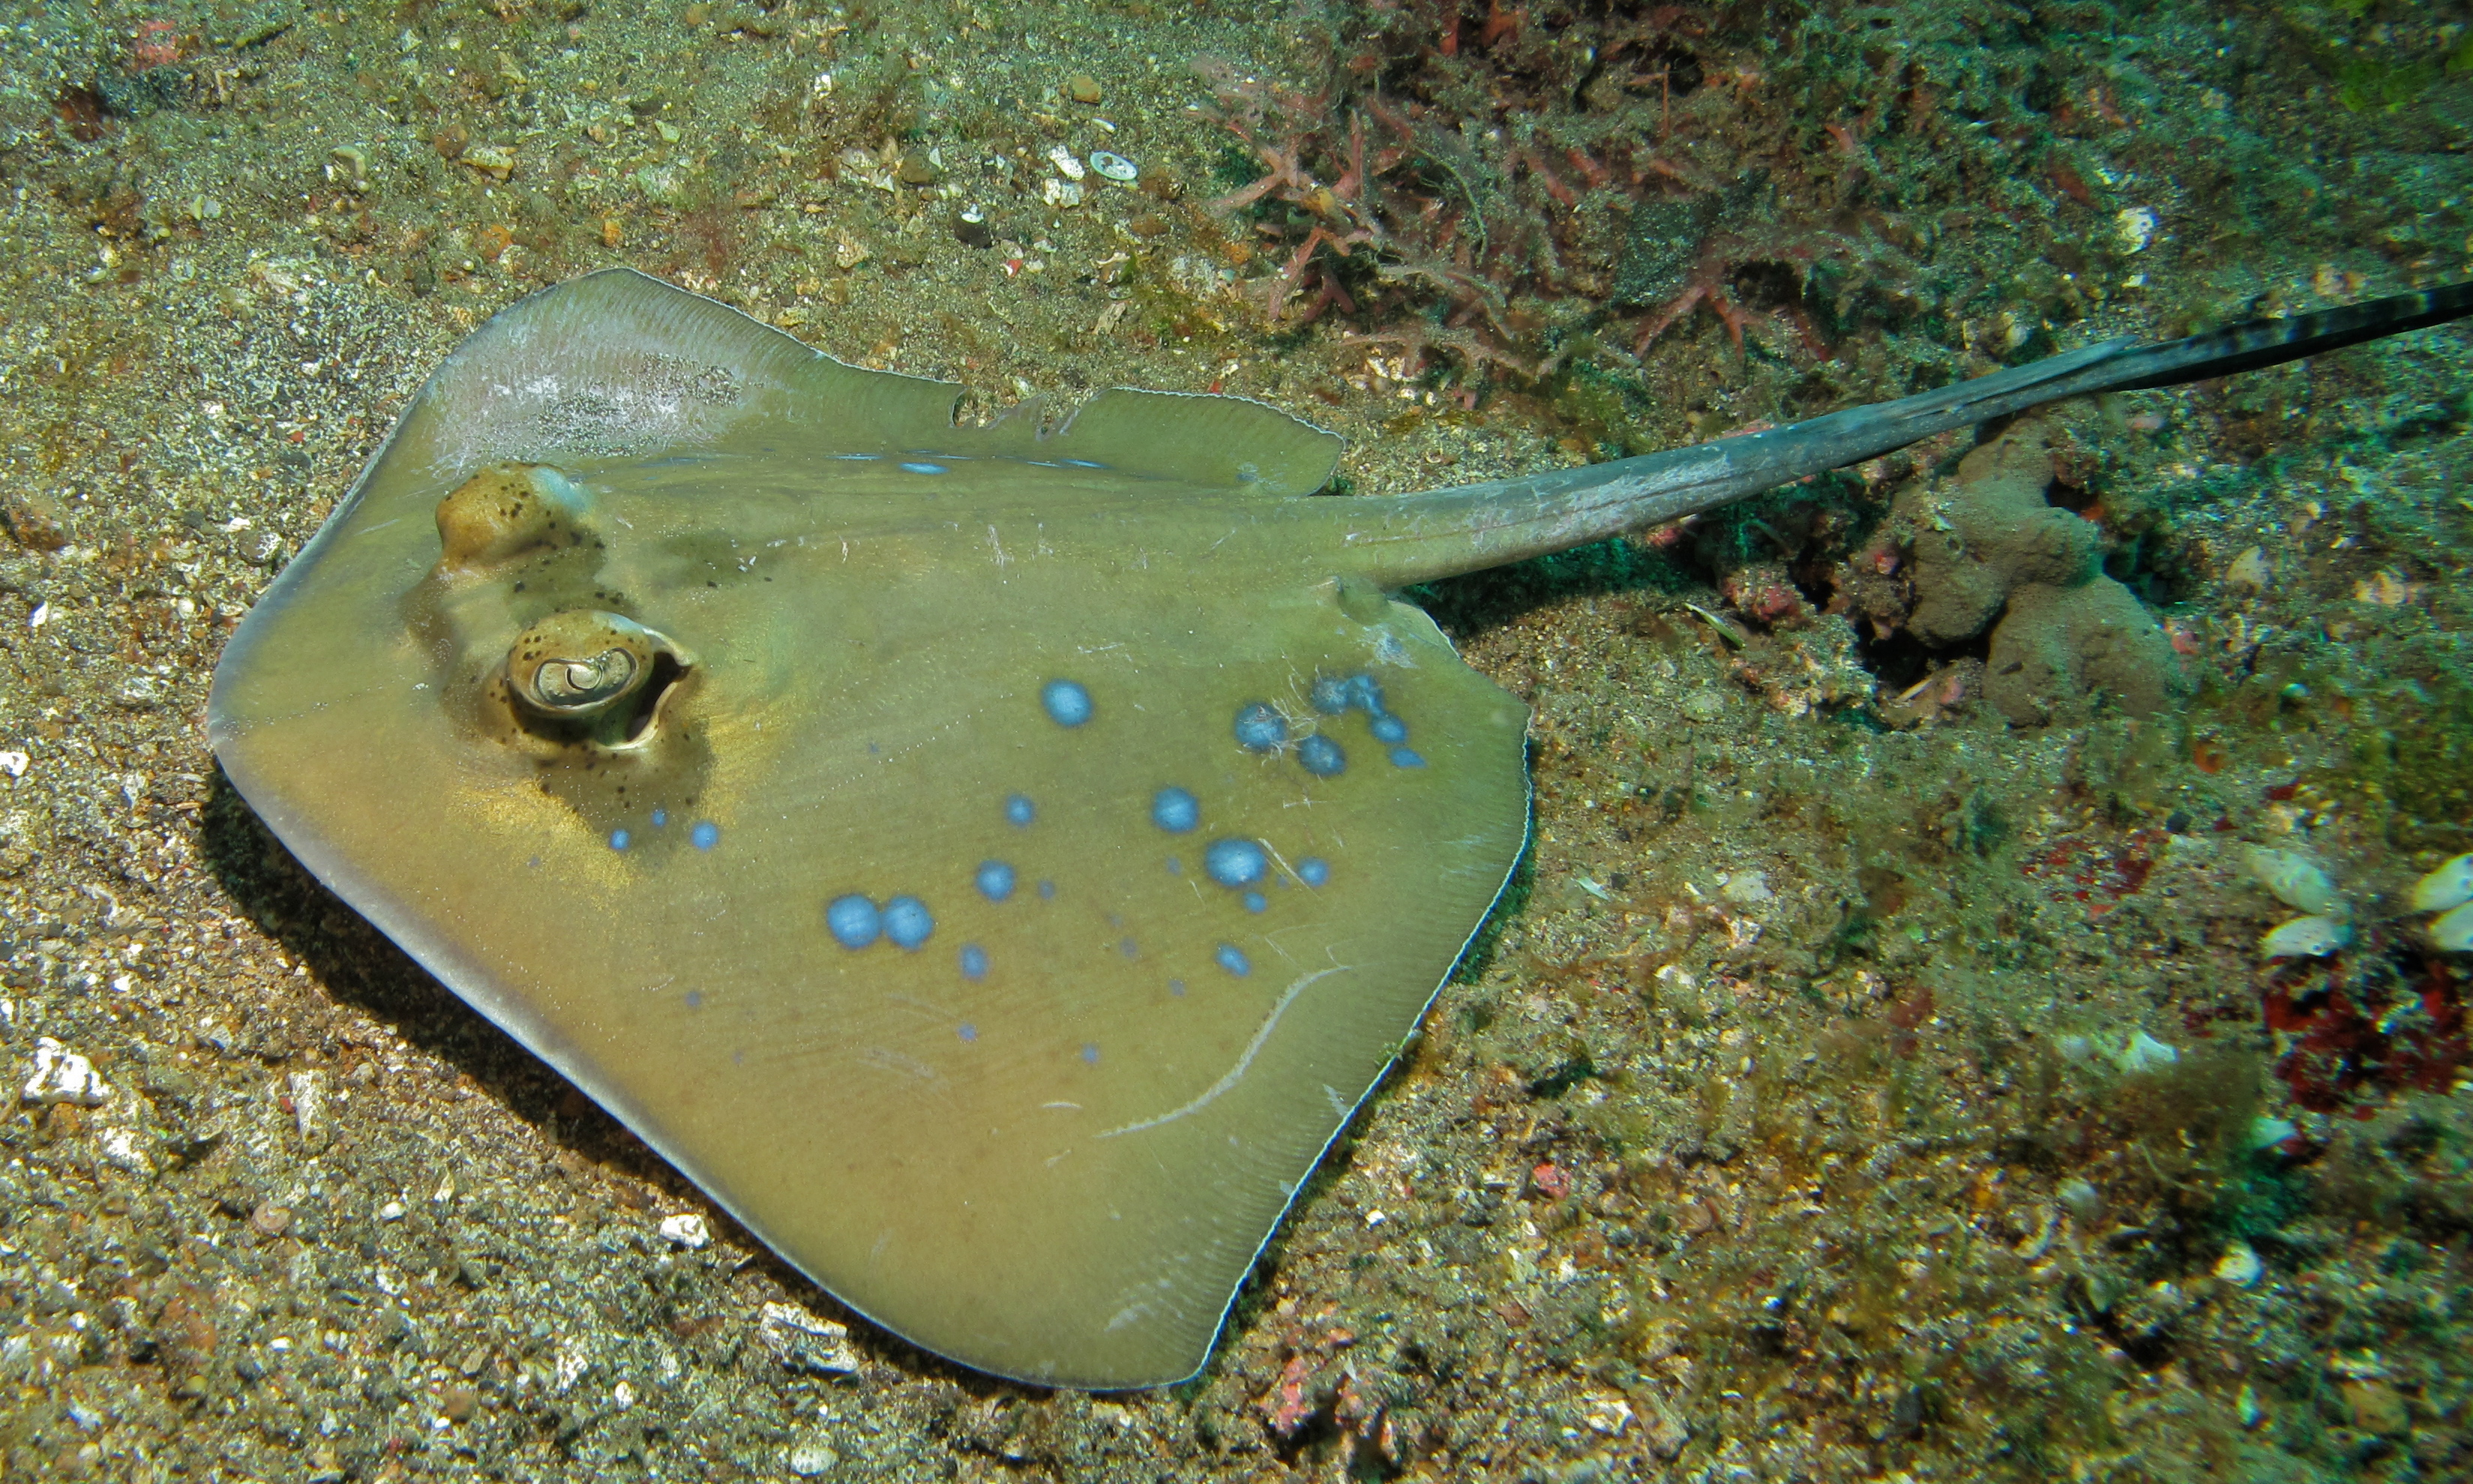
\includegraphics[width=0.5\linewidth]{Blue-spotted_Stingray_(Neotrygon_kuhlii)_(8465011759).jpg}
\end{center}
\caption{Here's a caption!}

 \end{figure}

\section{Formatting text and Writing an equation}

\textbf{Here is a bolded sentence}     
\newline
\textit{Here is an italicized sentence}     
\newline
\textit{\textbf{Here is a sentence that is bolded and italicized}}    
\newline
\textsc{Here is a sentence in small caps}   
\newline

Here's a pair of equations from coexistence theory:
\newline
$\frac{dN_{1}}{dt} = r_{1}N_{1} (1 - \alpha_{11}N_{1} - \alpha_{12}N_{2})$
$\frac{dN_{2}}{dt} = r_{2}N_{2} (1 - \alpha_{22}N_{2} - \alpha_{21}N_{1})$


\end{document}
